\documentclass[]{article}

\usepackage{graphicx,type1cm,eso-pic,color}
\usepackage[spanish]{babel} %%%% for


\makeatletter
          \AddToShipoutPicture{
            \setlength{\@tempdimb}{.95\paperwidth}
            \setlength{\@tempdimc}{.5\paperheight}
            \setlength{\unitlength}{1pt}
            \put(\strip@pt\@tempdimb,\strip@pt\@tempdimc){
        \makebox(0,0){\rotatebox{-90}{\textcolor[gray]{0.90}
        {\fontsize{.65cm}{.5cm}\selectfont{\rm Dae-Jin Lee}}}}
            }
        }
          \AddToShipoutPicture{
            \setlength{\@tempdimb}{.50\paperwidth}
            \setlength{\@tempdimc}{.95\paperheight}
            \setlength{\unitlength}{1pt}
            \put(\strip@pt\@tempdimb,\strip@pt\@tempdimc){
        \makebox(0,0){\rotatebox{0}{\textcolor[gray]{0.90}
        {\fontsize{.5cm}{.5cm}\selectfont{\rm Curso de Estad\'istica b\'asica para Data Scientist  - @datahack}}}}
            }
        }
\makeatother

\def\tightlist{}

\usepackage{lmodern}
\usepackage{amssymb,amsmath}
\usepackage{ifxetex,ifluatex}
\usepackage{fixltx2e} % provides \textsubscript
\ifnum 0\ifxetex 1\fi\ifluatex 1\fi=0 % if pdftex
  \usepackage[T1]{fontenc}
  \usepackage[utf8]{inputenc}
\else % if luatex or xelatex
  \ifxetex
    \usepackage{mathspec}
    \usepackage{xltxtra,xunicode}
  \else
    \usepackage{fontspec}
  \fi
  \defaultfontfeatures{Mapping=tex-text,Scale=MatchLowercase}
  \newcommand{\euro}{???}
\fi
% use upquote if available, for straight quotes in verbatim environments
\IfFileExists{upquote.sty}{\usepackage{upquote}}{}
% use microtype if available
\IfFileExists{microtype.sty}{%
\usepackage{microtype}
\UseMicrotypeSet[protrusion]{basicmath} % disable protrusion for tt fonts
}{}
\usepackage{color}
\usepackage{fancyvrb}
\newcommand{\VerbBar}{|}
\newcommand{\VERB}{\Verb[commandchars=\\\{\}]}
\DefineVerbatimEnvironment{Highlighting}{Verbatim}{commandchars=\\\{\}}
% Add ',fontsize=\small' for more characters per line
\usepackage{framed}
\definecolor{shadecolor}{RGB}{248,248,248}
\newenvironment{Shaded}{\begin{snugshade}}{\end{snugshade}}
\newcommand{\KeywordTok}[1]{\textcolor[rgb]{0.13,0.29,0.53}{\textbf{{#1}}}}
\newcommand{\DataTypeTok}[1]{\textcolor[rgb]{0.13,0.29,0.53}{{#1}}}
\newcommand{\DecValTok}[1]{\textcolor[rgb]{0.00,0.00,0.81}{{#1}}}
\newcommand{\BaseNTok}[1]{\textcolor[rgb]{0.00,0.00,0.81}{{#1}}}
\newcommand{\FloatTok}[1]{\textcolor[rgb]{0.00,0.00,0.81}{{#1}}}
\newcommand{\ConstantTok}[1]{\textcolor[rgb]{0.00,0.00,0.00}{{#1}}}
\newcommand{\CharTok}[1]{\textcolor[rgb]{0.31,0.60,0.02}{{#1}}}
\newcommand{\SpecialCharTok}[1]{\textcolor[rgb]{0.00,0.00,0.00}{{#1}}}
\newcommand{\StringTok}[1]{\textcolor[rgb]{0.31,0.60,0.02}{{#1}}}
\newcommand{\VerbatimStringTok}[1]{\textcolor[rgb]{0.31,0.60,0.02}{{#1}}}
\newcommand{\SpecialStringTok}[1]{\textcolor[rgb]{0.31,0.60,0.02}{{#1}}}
\newcommand{\ImportTok}[1]{{#1}}
\newcommand{\CommentTok}[1]{\textcolor[rgb]{0.56,0.35,0.01}{\textit{{#1}}}}
\newcommand{\DocumentationTok}[1]{\textcolor[rgb]{0.56,0.35,0.01}{\textbf{\textit{{#1}}}}}
\newcommand{\AnnotationTok}[1]{\textcolor[rgb]{0.56,0.35,0.01}{\textbf{\textit{{#1}}}}}
\newcommand{\CommentVarTok}[1]{\textcolor[rgb]{0.56,0.35,0.01}{\textbf{\textit{{#1}}}}}
\newcommand{\OtherTok}[1]{\textcolor[rgb]{0.56,0.35,0.01}{{#1}}}
\newcommand{\FunctionTok}[1]{\textcolor[rgb]{0.00,0.00,0.00}{{#1}}}
\newcommand{\VariableTok}[1]{\textcolor[rgb]{0.00,0.00,0.00}{{#1}}}
\newcommand{\ControlFlowTok}[1]{\textcolor[rgb]{0.13,0.29,0.53}{\textbf{{#1}}}}
\newcommand{\OperatorTok}[1]{\textcolor[rgb]{0.81,0.36,0.00}{\textbf{{#1}}}}
\newcommand{\BuiltInTok}[1]{{#1}}
\newcommand{\ExtensionTok}[1]{{#1}}
\newcommand{\PreprocessorTok}[1]{\textcolor[rgb]{0.56,0.35,0.01}{\textit{{#1}}}}
\newcommand{\AttributeTok}[1]{\textcolor[rgb]{0.77,0.63,0.00}{{#1}}}
\newcommand{\RegionMarkerTok}[1]{{#1}}
\newcommand{\InformationTok}[1]{\textcolor[rgb]{0.56,0.35,0.01}{\textbf{\textit{{#1}}}}}
\newcommand{\WarningTok}[1]{\textcolor[rgb]{0.56,0.35,0.01}{\textbf{\textit{{#1}}}}}
\newcommand{\AlertTok}[1]{\textcolor[rgb]{0.94,0.16,0.16}{{#1}}}
\newcommand{\ErrorTok}[1]{\textcolor[rgb]{0.64,0.00,0.00}{\textbf{{#1}}}}
\newcommand{\NormalTok}[1]{{#1}}
\usepackage{longtable,booktabs}
\usepackage{graphicx}
\makeatletter
\def\maxwidth{\ifdim\Gin@nat@width>\linewidth\linewidth\else\Gin@nat@width\fi}
\def\maxheight{\ifdim\Gin@nat@height>\textheight\textheight\else\Gin@nat@height\fi}
\makeatother
% Scale images if necessary, so that they will not overflow the page
% margins by default, and it is still possible to overwrite the defaults
% using explicit options in \includegraphics[width, height, ...]{}
\setkeys{Gin}{width=\maxwidth,height=\maxheight,keepaspectratio}
\ifxetex
  \usepackage[setpagesize=false, % page size defined by xetex
              unicode=false, % unicode breaks when used with xetex
              xetex]{hyperref}
\else
  \usepackage[unicode=true]{hyperref}
\fi
\hypersetup{breaklinks=true,
            bookmarks=true,
            pdfauthor={Dae-Jin Lee \textless{} lee.daejin@gmail.com \textgreater{}},
            pdftitle={Curso de Estadística básica para Data Scientists},
            colorlinks=true,
            citecolor=blue,
            urlcolor=blue,
            linkcolor=magenta,
            pdfborder={0 0 0}}
\urlstyle{same}  % don't use monospace font for urls
\setlength{\parindent}{0pt}
\setlength{\parskip}{6pt plus 2pt minus 1pt}
\setlength{\emergencystretch}{3em}  % prevent overfull lines
\setcounter{secnumdepth}{5}

\title{\textbf{Curso de Estadística básica para Data Scientists}}
\author{Dae-Jin Lee \textless{}
\href{mailto:lee.daejin@gmail.com}{\nolinkurl{lee.daejin@gmail.com}}
\textgreater{}}
\date{TEMA 5. Inferencia Estadística}

\usepackage{amsfonts}
\usepackage{amsmath}
\usepackage{amssymb}
\usepackage{natbib}
%\usepackage[T1]{fontenc}
\usepackage{latexsym}
\usepackage{graphicx}
\usepackage{caption}
\usepackage{subcaption}
\usepackage{color}
\usepackage{algorithm2e}
%%
%     Definitions
%
\newcommand{\tri}{\bigtriangleup}
\newcommand{\Xp}{X^\prime}
\newcommand{\E}{\mbox{E}}
\newcommand{\Hh}{\mbox{H}}
\newcommand{\V}{\mbox{Var}}
\newcommand{\tr}{\mbox{tr}}
\newcommand{\CV}{\mbox{CV}}
\newcommand{\GCV}{\mbox{GCV}}
\newcommand{\AIC}{\mbox{AIC}}
\newcommand{\ph}{\phantom{0}}
\newcommand{\half}{\mbox{${1\over2}$}}
\newcommand{\bfzero}{\boldsymbol{0}}
\newcommand{\bfone}{\boldsymbol{1}}

\newcommand{\bfa}{\boldsymbol{a}}
\newcommand{\bfb}{\boldsymbol{b}}
\newcommand{\bfe}{\boldsymbol{e}}
\newcommand{\bff}{\boldsymbol{f}}
\newcommand{\bfg}{\boldsymbol{g}}
\newcommand{\bfs}{\boldsymbol{s}}
\newcommand{\bfu}{\boldsymbol{u}}
\newcommand{\bfx}{\boldsymbol{x}}
\newcommand{\bfy}{\boldsymbol{y}}
\newcommand{\bfz}{\boldsymbol{z}}

\newcommand{\bfA}{\boldsymbol{A}}
\newcommand{\bfB}{\boldsymbol{B}}
\newcommand{\bfC}{\boldsymbol{C}}
\newcommand{\bfD}{\boldsymbol{D}}
\newcommand{\bfF}{\boldsymbol{F}}
\newcommand{\bfG}{\boldsymbol{G}}
\newcommand{\bfH}{\boldsymbol{H}}
\newcommand{\bfI}{\boldsymbol{I}}
\newcommand{\bfM}{\boldsymbol{M}}
\newcommand{\bfP}{\boldsymbol{P}}
\newcommand{\bfQ}{\boldsymbol{Q}}
\newcommand{\bfR}{\boldsymbol{R}}
\newcommand{\bfS}{\boldsymbol{S}}
\newcommand{\bfT}{\boldsymbol{T}}
\newcommand{\bfU}{\boldsymbol{U}}
\newcommand{\bfV}{\boldsymbol{V}}
\newcommand{\bfW}{\boldsymbol{W}}
\newcommand{\bfX}{\boldsymbol{X}}
\newcommand{\bfY}{\boldsymbol{Y}}
\newcommand{\bfZ}{\boldsymbol{Z}}


\newcommand{\bfalpha}{\boldsymbol{\alpha}}
\newcommand{\bfbeta}{\boldsymbol{\beta}}
\newcommand{\bfepsilon}{\boldsymbol{\epsilon}}
\newcommand{\bfgamma}{\boldsymbol{\gamma}}
\newcommand{\bfGamma}{\boldsymbol{\Gamma}}
\newcommand{\bfmu}{\boldsymbol{\mu}}
\newcommand{\bfeta}{\boldsymbol{\eta}}
\newcommand{\bfrho}{\boldsymbol{\rho}}
\newcommand{\bftheta}{\boldsymbol{\theta}}
\newcommand{\bfxi}{\boldsymbol{\xi}}
\newcommand{\bftau}{\boldsymbol{\tau}}
\newcommand{\bflambda}{\boldsymbol{\lambda}}
\newcommand{\bfsigma}{\boldsymbol{\sigma}}
\newcommand{\bfLambda}{\boldsymbol{\Lambda}}
\newcommand{\bfSigma}{\boldsymbol{\Sigma}}

\renewcommand{\theequation}{\thesection.\arabic{equation}}
\numberwithin{equation}{section}

\begin{document}
\maketitle

{
\hypersetup{linkcolor=black}
\setcounter{tocdepth}{2}
\tableofcontents
}
\newpage

\href{https://idaejin.github.io/bcam-courses/R/datahack/}{Regresar a la
página principal}

\section{Inferencia Estadística}\label{inferencia-estadistica}

La inferencia estadística permite obtener conclusiones a partir de los
datos. Hay muchas maneras de realizar inferencia incluyendo la
modelización estadística, estrategias orientadas a datos y uso explícito
de diseños y aleatorización en análisis de datos. Además, existen
teorías amplias (frecuencias, bayesianas, verosimilitud, , \ldots{}) y
numerosas dificultades (datos faltantes, sesgos) para realizar la
inferencia. Este tema presenta los fundamentos de la inferencia en un
enfoque práctico, con el fin de utilizar la inferencia estadística para
tomar decisiones informadas en el análisis de datos.

\subsection{Estimation por intervalos}\label{estimation-por-intervalos}

Es un requisito común para estimar eficientemente los parámetros de
población basados en datos de muestras aleatorias simples.

\begin{Shaded}
\begin{Highlighting}[]
\KeywordTok{library}\NormalTok{(MASS)}
\NormalTok{?survey}
\KeywordTok{head}\NormalTok{(survey)}
\end{Highlighting}
\end{Shaded}

\begin{verbatim}
##      Sex Wr.Hnd NW.Hnd W.Hnd    Fold Pulse    Clap Exer Smoke Height
## 1 Female   18.5   18.0 Right  R on L    92    Left Some Never 173.00
## 2   Male   19.5   20.5  Left  R on L   104    Left None Regul 177.80
## 3   Male   18.0   13.3 Right  L on R    87 Neither None Occas     NA
## 4   Male   18.8   18.9 Right  R on L    NA Neither None Never 160.00
## 5   Male   20.0   20.0 Right Neither    35   Right Some Never 165.00
## 6 Female   18.0   17.7 Right  L on R    64   Right Some Never 172.72
##        M.I    Age
## 1   Metric 18.250
## 2 Imperial 17.583
## 3     <NA> 16.917
## 4   Metric 20.333
## 5   Metric 23.667
## 6 Imperial 21.000
\end{verbatim}

\textbf{Estimación puntual de la media poblacional}

Para cualquier muestra aleatoria en particular, siempre podemos calcular
la media muestral. Aunque la mayoría de las veces no es la media real de
la población, sirve como una buena estimación puntual. Por ejemplo, en
los datos \texttt{survey}, la encuesta se realiza sobre una muestra de
la población estudiantil. Podemos calcular la media de la muestra y
utilizarla como una estimación del parámetro de población
correspondiente.

\textbf{Ejercicio:} Encuentra una estimación puntual de la altura media
de los estudiantes universitarios con los datos de la muestra de la
encuesta.

\begin{Shaded}
\begin{Highlighting}[]
\KeywordTok{mean}\NormalTok{(survey$Height)}
\end{Highlighting}
\end{Shaded}

\begin{verbatim}
## [1] NA
\end{verbatim}

\begin{Shaded}
\begin{Highlighting}[]
\KeywordTok{mean}\NormalTok{(survey$Height,}\DataTypeTok{na.rm=}\OtherTok{TRUE}\NormalTok{) }
\end{Highlighting}
\end{Shaded}

\begin{verbatim}
## [1] 172.3809
\end{verbatim}

\begin{Shaded}
\begin{Highlighting}[]
\CommentTok{# or}
\KeywordTok{mean}\NormalTok{(}\KeywordTok{na.omit}\NormalTok{(survey$Height))}
\end{Highlighting}
\end{Shaded}

\begin{verbatim}
## [1] 172.3809
\end{verbatim}

Una vez calculada uns estimación puntual de la media de la población,
necesitaríamos una manera de cuantificar su exactitud.

\subsubsection{Intervalo para la estimación de la media poblacinal (con
varianza
conocida)}\label{intervalo-para-la-estimacion-de-la-media-poblacinal-con-varianza-conocida}

Sea \(100~(1-\alpha/2)\) el percentile de la distribución Normal
estándar \(z_{\alpha/2}\). Para una muestra aleatoria de tamaño
suficientemente grande, la estimación del intervalo al nivel de
confianza \((1-\alpha/2)\) es: \[
  \bar{x} \pm \frac{\sigma}{\sqrt{n}}
\]

\textbf{Ejercicio:} supongamos una población de desviación típica
\(\sigma\) de las alturas de la encuesta es 9.48. Calcula el margen de
error y la estimación del intervalo de confianza del 95\%.

\begin{Shaded}
\begin{Highlighting}[]
\NormalTok{x <-}\StringTok{ }\KeywordTok{na.omit}\NormalTok{(survey$Height)}
\NormalTok{n <-}\StringTok{ }\KeywordTok{length}\NormalTok{(x)}
\NormalTok{sigma <-}\StringTok{ }\FloatTok{9.48}
\NormalTok{sem =}\StringTok{ }\NormalTok{sigma/}\KeywordTok{sqrt}\NormalTok{(n)  }\CommentTok{# Standard error of the mean}
\NormalTok{sem}
\end{Highlighting}
\end{Shaded}

\begin{verbatim}
## [1] 0.6557453
\end{verbatim}

Dado que hay dos colas de la distribución normal, el nivel de confianza
del 95\% implicaría el percentil 97.5 de la distribución normal en la
cola superior. Por tanto, \(z_{\alpha/2}\) viene dado por
\texttt{qnorm(.975)}. Lo multiplicamos con el error estándar de la media
\texttt{sem} y obtenemos el margen de error.

\begin{Shaded}
\begin{Highlighting}[]
\NormalTok{E <-}\StringTok{ }\KeywordTok{qnorm}\NormalTok{(}\FloatTok{0.975}\NormalTok{)*sem }
\NormalTok{E  }\CommentTok{# margin of error}
\end{Highlighting}
\end{Shaded}

\begin{verbatim}
## [1] 1.285237
\end{verbatim}

\begin{Shaded}
\begin{Highlighting}[]
\NormalTok{xbar <-}\StringTok{ }\KeywordTok{mean}\NormalTok{(x,}\DataTypeTok{na.rm =} \OtherTok{TRUE}\NormalTok{)}
\NormalTok{xbar +}\StringTok{ }\KeywordTok{c}\NormalTok{(-E,E)}
\end{Highlighting}
\end{Shaded}

\begin{verbatim}
## [1] 171.0956 173.6661
\end{verbatim}

De manera alternativa, podemos utilizar \texttt{z.test}

\begin{Shaded}
\begin{Highlighting}[]
\KeywordTok{library}\NormalTok{(TeachingDemos)}
\KeywordTok{z.test}\NormalTok{(x,}\DataTypeTok{sd=}\NormalTok{sigma)}
\end{Highlighting}
\end{Shaded}

\begin{verbatim}
## 
##  One Sample z-test
## 
## data:  x
## z = 262.88, n = 209.00000, Std. Dev. = 9.48000, Std. Dev. of the
## sample mean = 0.65575, p-value < 2.2e-16
## alternative hypothesis: true mean is not equal to 0
## 95 percent confidence interval:
##  171.0956 173.6661
## sample estimates:
## mean of x 
##  172.3809
\end{verbatim}

Suponiendo que la desviación estándar de la población \$ ~sigma \$ sea
9.48, el margen de error para la encuesta de altura del estudiante al
nivel de confianza del 95\% es 1.2852372 centímetros. El intervalo de
confianza está entre 171.095624 y 173.6660984 centimetros.

\subsubsection{Intervalo para la estimación de la media poblacinal (con
varianza
desconocida)}\label{intervalo-para-la-estimacion-de-la-media-poblacinal-con-varianza-desconocida}

\begin{Shaded}
\begin{Highlighting}[]
\NormalTok{s =}\StringTok{ }\KeywordTok{sd}\NormalTok{(x)}
\NormalTok{SE <-}\StringTok{ }\NormalTok{s/}\KeywordTok{sqrt}\NormalTok{(n)}
\NormalTok{E =}\StringTok{ }\KeywordTok{qt}\NormalTok{(.}\DecValTok{975}\NormalTok{, }\DataTypeTok{df=}\NormalTok{n}\DecValTok{-1}\NormalTok{)*SE; E}
\end{Highlighting}
\end{Shaded}

\begin{verbatim}
## [1] 1.342878
\end{verbatim}

\begin{Shaded}
\begin{Highlighting}[]
\NormalTok{xbar +}\StringTok{ }\KeywordTok{c}\NormalTok{(-E, E) }
\end{Highlighting}
\end{Shaded}

\begin{verbatim}
## [1] 171.0380 173.7237
\end{verbatim}

\begin{Shaded}
\begin{Highlighting}[]
\CommentTok{# or }

\KeywordTok{t.test}\NormalTok{(x)}
\end{Highlighting}
\end{Shaded}

\begin{verbatim}
## 
##  One Sample t-test
## 
## data:  x
## t = 253.07, df = 208, p-value < 2.2e-16
## alternative hypothesis: true mean is not equal to 0
## 95 percent confidence interval:
##  171.0380 173.7237
## sample estimates:
## mean of x 
##  172.3809
\end{verbatim}

Sin el suepuesto sobre la desviación estándar de la población, el margen
de error para la encuesta de altura del estudiante a un nivel de
confianza del 95\% es de 1.3429 centímetros. El intervalo de confianza
está entre 171.04 y 173.72 centímetros.

\paragraph{Tamaño muestral de la media
poblacional}\label{tamano-muestral-de-la-media-poblacional}

La calidad de una encuesta muestral puede mejorarse aumentando el tamaño
de la muestra. La fórmula siguiente proporciona el tamaño de muestra
requerido bajo el requisito de estimación del intervalo medio de la
población a \((1-\alpha)\) nivel de confianza, margen de error \(E\) y
varianza poblacional \(\sigma^2\). Aquí, \(z_{\alpha-2}\) es el
percentil \(100 (1 -\alpha/2)\) de la distribución normal estándar.

\[
    n = \frac{(z_{\alpha/2})^2 \sigma^2}{E^2}
\]

\textbf{Ejercicio:}

Supongamos que la desviación estándar de la población \(\sigma\) de la
altura del estudiante en \texttt{survey} es 9.48. Encuentre el tamaño de
muestra necesario para lograr un margen de error de 1,2 centímetros a un
nivel de confianza del 95\%.

\begin{Shaded}
\begin{Highlighting}[]
\NormalTok{zstar =}\StringTok{ }\KeywordTok{qnorm}\NormalTok{(.}\DecValTok{975}\NormalTok{) }
\NormalTok{sigma =}\StringTok{ }\FloatTok{9.48} 
\NormalTok{E =}\StringTok{ }\FloatTok{1.2} 
\NormalTok{zstar^}\DecValTok{2} \NormalTok{*sigma^}\DecValTok{2}\NormalTok{/}\StringTok{ }\NormalTok{E^}\DecValTok{2} 
\end{Highlighting}
\end{Shaded}

\begin{verbatim}
## [1] 239.7454
\end{verbatim}

Basándonos en la suposición de que la desviación estándar de la
población es de 9,48, necesita un tamaño de muestra de 240 para lograr
un margen de error de 1,2 centímetros con un nivel de confianza del
95\%.

\subsubsection{Estimación de intervalos de confianza para la proporción
poblacional}\label{estimacion-de-intervalos-de-confianza-para-la-proporcion-poblacional}

\textbf{Estimación puntual de la proporción poblacional}

Los cuestionarios de opción múltiple en una encuesta se usan a menudo
para determinar la proporción de una población con ciertas
características. Por ejemplo, podemos estimar la proporción de
estudiantes femeninas en la universidad sobre la base del resultado en
el conjunto de datos de muestra \texttt{survey}.

\textbf{Ejercicio:} Calcula una estimación puntual de la proporción de
estudiantes femeninos de la encuesta.

\begin{Shaded}
\begin{Highlighting}[]
\KeywordTok{library}\NormalTok{(MASS)}
\NormalTok{gender.response <-}\StringTok{ }\KeywordTok{na.omit}\NormalTok{(survey$Sex) }\CommentTok{# filter out NA's}
\NormalTok{n <-}\StringTok{ }\KeywordTok{length}\NormalTok{(gender.response)}
\KeywordTok{table}\NormalTok{(gender.response)}
\end{Highlighting}
\end{Shaded}

\begin{verbatim}
## gender.response
## Female   Male 
##    118    118
\end{verbatim}

Para averiguar el número de mujeres estudiantes, comparamos
\texttt{gender.response}

\begin{Shaded}
\begin{Highlighting}[]
\NormalTok{k <-}\StringTok{ }\KeywordTok{sum}\NormalTok{(gender.response ==}\StringTok{ "Female"}\NormalTok{) }
\CommentTok{# or }
\NormalTok{k <-}\StringTok{ }\KeywordTok{table}\NormalTok{(gender.response)[}\DecValTok{1}\NormalTok{]}

\NormalTok{pbar <-}\StringTok{ }\NormalTok{k/n; pbar}
\end{Highlighting}
\end{Shaded}

\begin{verbatim}
## Female 
##    0.5
\end{verbatim}

La estimación puntual de la proporción de estudiantes femeninas en la
encuesta es del 50\%.

Con el fin de calcular el intervalo de confianza de la proporción
estimada, denotemos el percentil \(100(1-\alpha/2)\) de la distribución
normal estándar como \(z_{\alpha/2}\). Si el tamaño de las muestras
\(n\) y la proporción de la población \(p\) satisfacen la condición de
que \(np \geq 5\) y \(n (1-p) \geq 5\), que los puntos finales de la
estimación del intervalo en \((1-\alpha)\) se define el nivel de
confianza en términos de la proporción de la muestra como sigue.

\[
      \bar{p} = \pm z_{\alpha/2} \sqrt{\frac{\bar{p}(1-\bar{p})}{n}} 
\]

Utilizaremos \texttt{prop.test}

\begin{Shaded}
\begin{Highlighting}[]
\KeywordTok{prop.test}\NormalTok{(k,n,}\DataTypeTok{conf.level =} \FloatTok{0.95}\NormalTok{)}
\end{Highlighting}
\end{Shaded}

\begin{verbatim}
## 
##  1-sample proportions test without continuity correction
## 
## data:  k out of n, null probability 0.5
## X-squared = 0, df = 1, p-value = 1
## alternative hypothesis: true p is not equal to 0.5
## 95 percent confidence interval:
##  0.4367215 0.5632785
## sample estimates:
##   p 
## 0.5
\end{verbatim}

A un nivel de confianza del 95\%, entre el 43,6\% y el 56,3\% de los
estudiantes universitarios son mujeres, y el margen de error es del
6,4\%.

\paragraph{Tamaño muestral de la proporción de la
población}\label{tamano-muestral-de-la-proporcion-de-la-poblacion}

La calidad de una encuesta muestral puede mejorarse aumentando el tamaño
de la muestra. La siguiente fórmula proporciona el tamaño de muestra
requerido bajo el requisito de estimación de intervalo de proporción de
poblacion a \((1-\alpha)\) nivel de confianza, margen de error \(E\), y
estimación de proporción planeada \(p\). Aquí, \(z_{\alpha/2}\) es el
percentil \(100(1-\alpha/2)\) de la distribución normal estándar.

\[
   n  = \frac{(z_{\alpha/2})^2 p (1-p)}{E^2}
\]

\begin{Shaded}
\begin{Highlighting}[]
\NormalTok{zstar =}\StringTok{ }\KeywordTok{qnorm}\NormalTok{(.}\DecValTok{975}\NormalTok{) }
\NormalTok{p =}\StringTok{ }\FloatTok{0.5} 
\NormalTok{E =}\StringTok{ }\FloatTok{0.05} 
\NormalTok{zstar^}\DecValTok{2} \NormalTok{*}\StringTok{ }\NormalTok{p *}\StringTok{ }\NormalTok{(}\DecValTok{1}\NormalTok{-p) /}\StringTok{ }\NormalTok{E^}\DecValTok{2} 
\end{Highlighting}
\end{Shaded}

\begin{verbatim}
## [1] 384.1459
\end{verbatim}

With a planned proportion estimate of 50\% at 95\% confidence level, it
needs a sample size of 385 to achieve a 5\% margin of error for the
survey of female student proportion.

\subsection{Inferencia sobre dos
poblaciones}\label{inferencia-sobre-dos-poblaciones}

A menudo es necesario sacar conclusiones sobre la diferencia entre dos
poblaciones por sus muestras de datos. En los siguientes tutoriales,
discutimos cómo estimar la diferencia de medios y proporciones entre dos
poblaciones de datos distribuidos normalmente.

\subsubsection{Media de población entre dos
muestras}\label{media-de-poblacion-entre-dos-muestras}

Se comparan dos muestras de datos si proceden de observaciones repetidas
del mismo sujeto. Aquí, suponemos que las poblaciones de datos siguen la
distribución normal. Usando un test-t para muestras pareadas
(\emph{paired t-test}), podemos obtener una estimación de intervalo de
la diferencia de los medios de población.

\begin{Shaded}
\begin{Highlighting}[]
\KeywordTok{library}\NormalTok{(MASS)}
\KeywordTok{data}\NormalTok{(immer)}
\NormalTok{?immer}
\KeywordTok{head}\NormalTok{(immer)}
\end{Highlighting}
\end{Shaded}

\begin{verbatim}
##   Loc Var    Y1    Y2
## 1  UF   M  81.0  80.7
## 2  UF   S 105.4  82.3
## 3  UF   V 119.7  80.4
## 4  UF   T 109.7  87.2
## 5  UF   P  98.3  84.2
## 6   W   M 146.6 100.4
\end{verbatim}

\textbf{Ejercicio:}

Suponiendo que los datos de \texttt{immer} siguen la distribución
normal, encuentre la estimación del intervalo de confianza del 95\% de
la diferencia entre los rendimientos medios de cebada entre los años
1931 y 1932.

\begin{Shaded}
\begin{Highlighting}[]
\KeywordTok{t.test}\NormalTok{(immer$Y1, immer$Y2, }\DataTypeTok{paired=}\OtherTok{TRUE}\NormalTok{) }
\end{Highlighting}
\end{Shaded}

\begin{verbatim}
## 
##  Paired t-test
## 
## data:  immer$Y1 and immer$Y2
## t = 3.324, df = 29, p-value = 0.002413
## alternative hypothesis: true difference in means is not equal to 0
## 95 percent confidence interval:
##   6.121954 25.704713
## sample estimates:
## mean of the differences 
##                15.91333
\end{verbatim}

\textbf{Answer:}

Entre los años 1931 y 1932 en el conjunto de datos \texttt{immer}, el
intervalo de confianza del 95\% de la diferencia en las medias de los
rendimientos de la cebada es el intervalo entre 6.122 y 25.705.

\subsection{Media poblacional entre dos muestras
independientes}\label{media-poblacional-entre-dos-muestras-independientes}

Dos muestras de datos son independientes si provienen de poblaciones no
relacionadas y las muestras no se afectan entre sí. Ahora, supondremos
que las poblaciones de datos siguen la distribución normal. Utilizando
la prueba \(t\) no pareada, podemos obtener una estimación de intervalo
de la diferencia entre dos medios poblacionales.

\emph{Ejemplo:}

En la columna de datos mpg columna del conjunto de datos
\texttt{mtcars}, hay datos de kilometraje de gas de varios 1974 EE.UU.
automóviles. \texttt{am} variable indica el tipo de transmisión del
modelo de automóvil (0 = automático, 1 = manual).

En particular, el consumo de gas para las transmisiones manuales y
automáticas son dos poblaciones de datos independientes.

\textbf{Ejercicio:}

Suponiendo que los datos en \texttt{mtcars} sigue la distribución
normal, encuentre la estimación del intervalo de confianza del 95\% de
la diferencia entre el consumo medio de gas de las transmisiones
manuales y automáticas.

\begin{Shaded}
\begin{Highlighting}[]
\KeywordTok{t.test}\NormalTok{(mpg ~}\StringTok{ }\NormalTok{am, }\DataTypeTok{data=}\NormalTok{mtcars) }
\end{Highlighting}
\end{Shaded}

\begin{verbatim}
## 
##  Welch Two Sample t-test
## 
## data:  mpg by am
## t = -3.7671, df = 18.332, p-value = 0.001374
## alternative hypothesis: true difference in means is not equal to 0
## 95 percent confidence interval:
##  -11.280194  -3.209684
## sample estimates:
## mean in group 0 mean in group 1 
##        17.14737        24.39231
\end{verbatim}

En \texttt{mtcars}, el kilometraje medio de la transmisión automática es
17.147 \texttt{mpg} y la transmisión manual es 24.392 \texttt{mpg}. El
intervalo de confianza del 95\% de la diferencia en el kilometraje medio
del gas está entre 3.2097 y 11.2802 \texttt{mpg}.

\subsection{Comparación de dos proporciones en una
población}\label{comparacion-de-dos-proporciones-en-una-poblacion}

Una encuesta realizada en dos poblaciones distintas producirá resultados
diferentes. A menudo es necesario comparar la proporción de la respuesta
de la encuesta entre las dos poblaciones. Aquí, suponemos que las
poblaciones de datos siguen la distribución normal.

\textbf{Ejericio:}

Los datos \texttt{quine}, contiene datos de los niños de una ciudad
australiana que se clasifican por origen étnico, género, edad, estado de
aprendizaje y el número de días ausentes de la escuela.

\begin{Shaded}
\begin{Highlighting}[]
\KeywordTok{library}\NormalTok{(MASS)}
\KeywordTok{data}\NormalTok{(quine)}
\NormalTok{?quine}
\KeywordTok{head}\NormalTok{(quine)}
\end{Highlighting}
\end{Shaded}

\begin{verbatim}
##   Eth Sex Age Lrn Days
## 1   A   M  F0  SL    2
## 2   A   M  F0  SL   11
## 3   A   M  F0  SL   14
## 4   A   M  F0  AL    5
## 5   A   M  F0  AL    5
## 6   A   M  F0  AL   13
\end{verbatim}

La columna \texttt{Eth} indica si el estudiante es aborigen o no
(\texttt{A} o \texttt{N}), y la columna \texttt{Sexo} indica el sexo
masculino o femenino (\texttt{M} o \texttt{F}).

\begin{Shaded}
\begin{Highlighting}[]
\KeywordTok{table}\NormalTok{(quine$Eth,quine$Sex)}
\end{Highlighting}
\end{Shaded}

\begin{verbatim}
##    
##      F  M
##   A 38 31
##   N 42 35
\end{verbatim}

\textbf{Ejercicio:}

Suponiendo que los datos en quine siguen la distribución normal,
encuentre la estimación del intervalo de confianza del 95\% de la
diferencia entre la proporción femenina de estudiantes aborígenes y la
proporción femenina de estudiantes no aborígenes, cada uno dentro de su
propio grupo étnico.

\textbf{Solución}

Aplicamos la función \texttt{prop.test} para calcular la diferencia en
las proporciones femeninas.

\begin{Shaded}
\begin{Highlighting}[]
\KeywordTok{prop.test}\NormalTok{(}\KeywordTok{table}\NormalTok{(quine$Eth, quine$Sex), }\DataTypeTok{correct=}\OtherTok{FALSE}\NormalTok{) }
\end{Highlighting}
\end{Shaded}

\begin{verbatim}
## 
##  2-sample test for equality of proportions without continuity
##  correction
## 
## data:  table(quine$Eth, quine$Sex)
## X-squared = 0.0040803, df = 1, p-value = 0.9491
## alternative hypothesis: two.sided
## 95 percent confidence interval:
##  -0.1564218  0.1669620
## sample estimates:
##    prop 1    prop 2 
## 0.5507246 0.5454545
\end{verbatim}

La estimación del intervalo de confianza del 95\% de la diferencia entre
la proporción femenina de estudiantes aborígenes y la proporción
femenina de estudiantes no aborígenes oscila entre -15,6\% y 16,7\%.

\subsection{Bondad de ajuste}\label{bondad-de-ajuste}

Se observa que muchas cantidades estadísticas derivadas de muestras de
datos siguen la distribución de Chi cuadrado. Por lo tanto podemos
usarlo para probar si una población se ajusta a una distribución de
probabilidad teórica particular.

\subsection{Prueba Chi-cuadrada de la
independencia}\label{prueba-chi-cuadrada-de-la-independencia}

Dos variables aleatorias \(x\) y \(y\) se llaman independientes si la
distribución de probabilidad de una variable no es afectada por la
presencia de otra. Supongamos que \$f\_ \{ij\} \$ es el recuento de
frecuencia observada de los eventos que pertenecen a la categoría
\(i\)-th de x y la categoría \(j\) -th de \(y\). También suponga que
\(e_{ij}\) sea el recuento esperado correspondiente si \(x\) y \(y\) son
independientes. La hipótesis nula de la suposición de la independencia
debe ser rechazada si el \(p\)-valor de las siguientes estadísticas de
la prueba de Chi cuadrado es menor que un nivel de significación dado
\(\alpha\).

\[
  \chi^2 = \sum_{i,j}\frac{(f_i - e_i)^2}{e_i}
\]

\textbf{Example:}

Del data set \texttt{survey}, La columna \texttt{Smoke} registra el
hábito de fumar de los estudiantes, mientras que la columna\texttt{Exer}
registra su nivel de ejercicio. Los valores permitidos en \texttt{Smoke}
son ``Heavy'', ``Regul'' (regularmente), ``Occas'' (ocasionalmente) y
``Never''. En cuanto a \texttt{Exer}, son ``Freq'' (frecuentemente),
``Algunos'' y ``Ninguno''.

\begin{Shaded}
\begin{Highlighting}[]
\KeywordTok{library}\NormalTok{(MASS)}
\KeywordTok{data}\NormalTok{(survey)}
\NormalTok{tbl <-}\StringTok{ }\KeywordTok{table}\NormalTok{(survey$Smoke,survey$Exer)}
\NormalTok{tbl}
\end{Highlighting}
\end{Shaded}

\begin{verbatim}
##        
##         Freq None Some
##   Heavy    7    1    3
##   Never   87   18   84
##   Occas   12    3    4
##   Regul    9    1    7
\end{verbatim}

\textbf{Ejercicio:}

Pruebe la hipótesis de si el hábito de fumar de los estudiantes es
independiente de su nivel de ejercicio con un nivel de significación de
\(0.05\).

\begin{Shaded}
\begin{Highlighting}[]
\NormalTok{chi2test <-}\StringTok{ }\KeywordTok{chisq.test}\NormalTok{(tbl) }
\NormalTok{chi2test}
\end{Highlighting}
\end{Shaded}

\begin{verbatim}
## 
##  Pearson's Chi-squared test
## 
## data:  tbl
## X-squared = 5.4885, df = 6, p-value = 0.4828
\end{verbatim}

Como el valor de p es 0.4828422 mayor que el nivel de significancia
0.05, no rechazamos la hipótesis nula de que el hábito de fumar es
independiente del nivel de ejercicio de los estudiantes.

El mensaje de \texttt{warning} que se encuentra en la solución anterior
se debe a los valores de celdas pequeñas en la tabla de contingencia.
Para evitar dicha advertencia, combinamos la segunda y tercera columnas
de \texttt{tbl} y la guardamos en una nueva tabla
denominada\texttt{ctbl}. A continuación, aplicamos la función
\texttt{chisq.test} en lugar de\texttt{ctbl}.

\begin{Shaded}
\begin{Highlighting}[]
\NormalTok{ctbl <-}\StringTok{ }\KeywordTok{cbind}\NormalTok{(tbl[,}\StringTok{"Freq"}\NormalTok{], tbl[,}\StringTok{"None"}\NormalTok{] +}\StringTok{ }\NormalTok{tbl[,}\StringTok{"Some"}\NormalTok{])}
\NormalTok{ctbl}
\end{Highlighting}
\end{Shaded}

\begin{verbatim}
##       [,1] [,2]
## Heavy    7    4
## Never   87  102
## Occas   12    7
## Regul    9    8
\end{verbatim}

\begin{Shaded}
\begin{Highlighting}[]
\NormalTok{chi2test <-}\StringTok{ }\KeywordTok{chisq.test}\NormalTok{(ctbl)}
\NormalTok{chi2test}
\end{Highlighting}
\end{Shaded}

\begin{verbatim}
## 
##  Pearson's Chi-squared test
## 
## data:  ctbl
## X-squared = 3.2328, df = 3, p-value = 0.3571
\end{verbatim}

El p-valor es 0.3571031 también mayor que el nivel de significancia
0.05.

\subsection{Test de U Mann-Whitney}\label{test-de-u-mann-whitney}

También conocida como Mann-Whitney-Wilcoxon (MWW), la prueba de suma de
Wilcoxon o Wilcoxon-Mann-Whitney es una prueba no paramétrica de la
hipótesis nula de que dos muestras provienen de la misma población de
muestra frente a una hipótesis alternativa, que una determinada
población tiende a tener valores más grandes que la otra. Es la prueba
alternativa a la prueba t de muestra independiente. Como prueba no
paramétrica, no asume ninguna suposición relacionada con la
distribución. Por lo tanto, podemos decidir si las distribuciones de la
población son idénticas sin suponer que sigan la distribución normal.

Hay, sin embargo, algunas suposiciones que se asumen:

\begin{enumerate}
\def\labelenumi{\arabic{enumi}.}
\tightlist
\item
  La muestra tomada de la población es aleatoria.
\item
  Se asume la independencia dentro de las muestras y la independencia
  mutua.
\item
  Se asume la escala de medida ordinaria.
\end{enumerate}

El test de U Mann-Whitney se utiliza en muchas áreas, pero sobre todo en
psicología, medicina/enfermería y en economía. Por ejemplo, en
psicología, se utiliza para comparar la actitud o comportamiento, etc.
En la medicina, se utiliza para conocer el efecto de dos medicamentos y
si son iguales o no. También se utiliza para saber si un medicamento en
particular cura o no la enfermedad. En economía de la empresa, se puede
utilizar para conocer las preferencias de diferentes personas y se puede
utilizar para ver si eso cambia dependiendo de la ubicación.

\textbf{Ejemplo:} Considera el conjunto de datos de \texttt{mtcars}.
Nuestro objetivo es averiguar si los automóviles de transmisión
automática son menos eficientes en comparación con los coches de
transmisión manual. Desde 1950, la mayoría de los coches vendidos en
Norteamérica han estado disponibles con una transmisión automática.

El conjunto de datos de \texttt{mtcars} procede de la revista ``Motor
Trend US'' de 1974, que consta de medidas de consumo de combustible
(mpg) y 10 aspectos diferentes del diseño y rendimiento de automóviles
para 32 automóviles (modelos 1973-74).

Primero representamos los datos (\texttt{mpg\ vs\ transmission}) con un
boxplot

\begin{Shaded}
\begin{Highlighting}[]
\KeywordTok{boxplot}\NormalTok{(mpg~am,}\DataTypeTok{data=}\NormalTok{mtcars,}\DataTypeTok{names=}\KeywordTok{c}\NormalTok{(}\StringTok{"automatic"}\NormalTok{,}\StringTok{"manual"}\NormalTok{),}\DataTypeTok{ylab=}\StringTok{"mpg"}\NormalTok{,}\DataTypeTok{xlab=}\StringTok{"Transmission"}\NormalTok{)}
\end{Highlighting}
\end{Shaded}

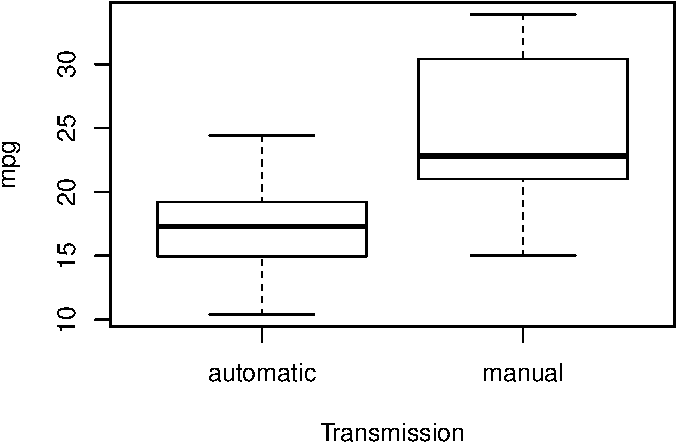
\includegraphics{tema5_files/figure-latex/unnamed-chunk-21-1.pdf}

o también como un gráfico de barras con errors

\begin{Shaded}
\begin{Highlighting}[]
\NormalTok{##### Step 1. reorganize the data in a correct format for statistical analysis}
\NormalTok{aggmpg <-}\StringTok{ }\KeywordTok{tapply}\NormalTok{(mtcars$mpg, mtcars$am, mean, }\DataTypeTok{na.rm =} \OtherTok{TRUE}\NormalTok{)}
\NormalTok{sdmpg <-}\StringTok{ }\KeywordTok{tapply}\NormalTok{(mtcars$mpg, mtcars$am, sd, }\DataTypeTok{na.rm =} \OtherTok{TRUE}\NormalTok{)}
\NormalTok{aggam <-}\StringTok{ }\KeywordTok{unique}\NormalTok{(}\KeywordTok{factor}\NormalTok{(}\KeywordTok{c}\NormalTok{(}\StringTok{"automatic"}\NormalTok{, }\StringTok{"manual"}\NormalTok{)))}
\NormalTok{##### Step 2. Plot a barchart}
\NormalTok{barmpg <-}\StringTok{ }\KeywordTok{barplot}\NormalTok{(aggmpg, }\DataTypeTok{names =} \NormalTok{aggam, }\DataTypeTok{ylim =} \KeywordTok{c}\NormalTok{(}\DecValTok{0}\NormalTok{, }\DecValTok{35}\NormalTok{), }\DataTypeTok{main =} \KeywordTok{paste}\NormalTok{(}\StringTok{"Average miles per gallon by transmission type"}\NormalTok{), }
    \DataTypeTok{space =} \FloatTok{0.3}\NormalTok{, }\DataTypeTok{axes =} \OtherTok{TRUE}\NormalTok{, }\DataTypeTok{axis.lty =} \DecValTok{10}\NormalTok{, }\DataTypeTok{col =} \StringTok{"white"}\NormalTok{, }\DataTypeTok{ylab =} \StringTok{"mpg"}\NormalTok{)}
\CommentTok{# put the plot in a box}
\KeywordTok{box}\NormalTok{()}
\CommentTok{# plot the vertical lines of the error bars}
\KeywordTok{segments}\NormalTok{(barmpg, aggmpg -}\StringTok{ }\NormalTok{sdmpg, barmpg, aggmpg +}\StringTok{ }\NormalTok{sdmpg, }\DataTypeTok{lwd =} \DecValTok{2}\NormalTok{)}
\CommentTok{# now plot the horizontal bounds for the error bars the lower bar}
\KeywordTok{segments}\NormalTok{(barmpg -}\StringTok{ }\FloatTok{0.05}\NormalTok{, aggmpg -}\StringTok{ }\NormalTok{sdmpg, barmpg +}\StringTok{ }\FloatTok{0.05}\NormalTok{, aggmpg -}\StringTok{ }\NormalTok{sdmpg, }\DataTypeTok{lwd =} \DecValTok{1}\NormalTok{)}
\CommentTok{# the upper bar}
\KeywordTok{segments}\NormalTok{(barmpg -}\StringTok{ }\FloatTok{0.05}\NormalTok{, aggmpg +}\StringTok{ }\NormalTok{sdmpg, barmpg +}\StringTok{ }\FloatTok{0.05}\NormalTok{, aggmpg +}\StringTok{ }\NormalTok{sdmpg, }\DataTypeTok{lwd =} \DecValTok{1}\NormalTok{)}
\end{Highlighting}
\end{Shaded}

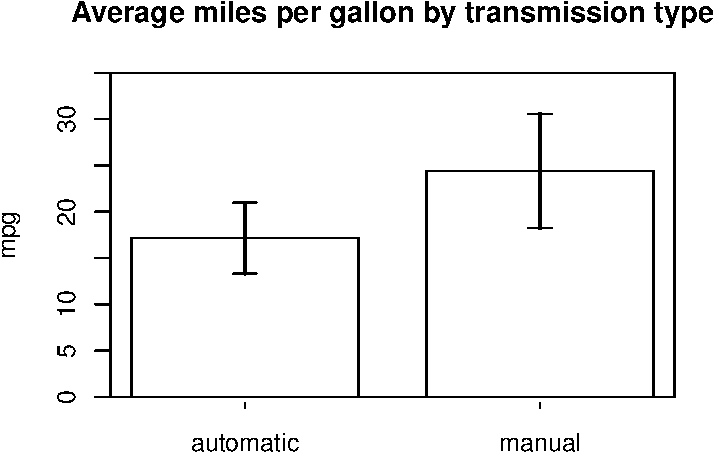
\includegraphics{tema5_files/figure-latex/unnamed-chunk-22-1.pdf}

Hacemos algunas pruebas estadísticas para comparar el mpg entre autos
automáticos y manuales.

La primera es un \(t\)-test, suponiendo que los datos de kilometraje
tienen una distribución normal. El resultado de la prueba demuestra
claramente que los coches de transmisión manual son más eficientes que
los automóviles de transmisión automática (millas por galón: 24,39
frente a 17,15).

\begin{Shaded}
\begin{Highlighting}[]
\KeywordTok{t.test}\NormalTok{(mpg ~}\StringTok{ }\KeywordTok{factor}\NormalTok{(am), }\DataTypeTok{data =} \NormalTok{mtcars)}
\end{Highlighting}
\end{Shaded}

\begin{verbatim}
## 
##  Welch Two Sample t-test
## 
## data:  mpg by factor(am)
## t = -3.7671, df = 18.332, p-value = 0.001374
## alternative hypothesis: true difference in means is not equal to 0
## 95 percent confidence interval:
##  -11.280194  -3.209684
## sample estimates:
## mean in group 0 mean in group 1 
##        17.14737        24.39231
\end{verbatim}

Sin embargo, la hipótesis de normalidad podría ser bastante fuerte, dado
el hecho de que no sabemos las verdaderas distribuciones subyacentes de
los datos de \texttt{mpg}. Además, el número de puntos de datos no es lo
suficientemente grande como para aplicar el teorema del límite central.
Por lo tanto, una prueba más conservadora sería la prueba de Wilcoxon,
con la hipótesis nula de que los datos de consumo de gas de las
transmisiones manuales y automáticas son de poblaciones idénticas.

\begin{Shaded}
\begin{Highlighting}[]
\KeywordTok{wilcox.test}\NormalTok{(mpg ~}\StringTok{ }\NormalTok{am, }\DataTypeTok{data =} \NormalTok{mtcars)}
\end{Highlighting}
\end{Shaded}

\begin{verbatim}
## Warning in wilcox.test.default(x = c(21.4, 18.7, 18.1, 14.3, 24.4, 22.8, :
## cannot compute exact p-value with ties
\end{verbatim}

\begin{verbatim}
## 
##  Wilcoxon rank sum test with continuity correction
## 
## data:  mpg by am
## W = 42, p-value = 0.001871
## alternative hypothesis: true location shift is not equal to 0
\end{verbatim}

Un test no paramétrico de Wilcoxon también rechaza la hipótesis nula de
que los datos de kilometraje de las transmisiones manuales y automáticas
son de la misma población (lo que indica una diferencia).

\subsection{Contrastes de hipótesis}\label{contrastes-de-hipotesis}

Deseamos probar una hipótesis nula (\(H_0\)) con una hipótesis
alternativa (\(H_1\)) usando un conjunto de datos. Las dos hipótesis
especifican dos modelos estadísticos para el proceso que produjo los
datos. La hipótesis alternativa es lo que esperamos que sea cierto si la
hipótesis nula es falsa. No podemos probar que la hipótesis alternativa
es verdadera, pero podemos demostrar que la alternativa es mucho más
plausible que la hipótesis nula dada a los datos. Esta demostración se
expresa generalmente en términos de una probabilidad (un valor de P) que
cuantifica la fuerza de la evidencia contra la hipótesis nula en favor
de la alternativa.

Nos preguntamos si los datos parecen ser consistentes con la hipótesis
nula o si es sería poco probable que obtuviera datos de este tipo si la
hipótesis nula fuera verídica, que al menos una de las dos hipótesis es
verdadera. Tratamos esta pregunta calculando la valor de una estadística
de prueba, es decir, una función de valor real particular de los datos.
Decidir si el valor de la estadística de prueba es consistente con la
hipótesis nula, necesitamos saber qué muestreo a esperar en nuestra
estadística de prueba si la hipótesis nula es verdadera. En otra las
palabras, necesitamos conocer la distribución nula, la distribución del
estadístico de prueba cuando la hipótesis nula es verdadera. En muchas
aplicaciones, la estadística de prueba se define de modo que su valor
nulo distribución es una distribución ``nombrada'' para la cual las
tablas son ampliamente accesibles; por ejemplo, el distribución normal
estándar, la distribución binomial con \(n = 100\) y \(p = 1/2\), la
distribución \(t\) con 4 grados de libertad, la distribución
chi-cuadrada con 23 grados de libertad, la distribución F con 2 y 20
grados de libertad.

Ahora, dado el valor de la estadística de prueba (un número), y la
distribución nula de la prueba estadística (una distribución teórica
generalmente representada por una densidad de probabilidad), queremos
ver si la estadística de la prueba está en el medio de la distribución
(consistente con el nulo hipótesis) o en una cola de la distribución
(haciendo que la hipótesis alternativa parezca más plausible). A veces
queremos considerar la cola derecha, a veces la mano izquierda cola, ya
veces ambas colas, dependiendo de cómo la estadística de prueba y la
hipótesis alternativa están definidos. Supongamos que los grandes
valores positivos de la estadística de prueba parecen más plausibles
bajo la hipótesis alternativa que bajo la hipótesis nula. Entonces
queremos una medida de qué tan lejos está nuestra estadística de prueba
en la cola derecha de la distribución nula. El \(p\)-valor proporciona
una medida de esta distancia. El \(p\)-valor (en esta situación) es la
probabilidad de que derecha de nuestra estadística de prueba calculada
usando la distribución nula. Cuanto más lejos de la prueba estadística
está en la cola, menor es el P-valor, y más fuerte es la evidencia
contra el nulo hipótesis a favor de la alternativa.

El \(p\)-valor puede interpretarse en términos de una hipotética
repetición del estudio. Suponer la hipótesis nula es verdadera y se
obtiene un nuevo conjunto de datos independientemente del primer
conjunto de datos pero utilizando el mismo procedimiento de muestreo. Si
el nuevo conjunto de datos se utiliza para calcular un nuevo valor de la
estadística de prueba (misma fórmula pero nuevos datos), ¿cuál es la
probabilidad de que el nuevo valor será más lejos en la cola (suponiendo
una prueba de una cola) que el valor original? este es el \(p\)-valor.

El \(p\)-valor suele interpretarse incorrectamente como la probabilidad
de que la hipótesis nula sea cierto. Trata de no cometer este error. En
una interpretación frecuentista de la probabilidad, no hay nada al azar
si la hipótesis es verdadera, la aleatoriedad está en el proceso
generando los datos. Se puede interpretar ``la probabilidad de que la
hipótesis nula sea verdadera'' usando probabilidad subjetiva, una medida
de la creencia de uno de que la hipótesis nula es verdadera. Se puede
calcular esta probabilidad subjetiva especificando una probabilidad
previa (creencia subjetiva antes de mirar los datos) que la hipótesis
nula es verdadera, y luego usar los datos y la modelo para actualizar la
probabilidad subjetiva de uno. Esto se denomina enfoque bayesiano porque
El teorema de Bayes se utiliza para actualizar las probabilidades
subjetivas para reflejar nueva información.

Al notificar un \(p\)-valor a personas que no están familiarizadas con
las estadísticas, a menudo es lenguaje descriptivo para indicar la
fuerza de la evidencia.

\begin{longtable}[]{@{}cc@{}}
\toprule
\begin{minipage}[b]{0.14\columnwidth}\centering\strut
\(p\)-value\strut
\end{minipage} & \begin{minipage}[b]{0.80\columnwidth}\centering\strut
Interpretacion\strut
\end{minipage}\tabularnewline
\midrule
\endhead
\begin{minipage}[t]{0.14\columnwidth}\centering\strut
\(p> 0.10\)\strut
\end{minipage} & \begin{minipage}[t]{0.80\columnwidth}\centering\strut
Ninguna evidencia contra la hipótesis nula. Los datos parecen ser
coherentes con la hipótesis nula\strut
\end{minipage}\tabularnewline
\begin{minipage}[t]{0.14\columnwidth}\centering\strut
\(0.05<p<0.10\)\strut
\end{minipage} & \begin{minipage}[t]{0.80\columnwidth}\centering\strut
Evidencia débil contra la hipótesis nula en favor de la
alternativa\strut
\end{minipage}\tabularnewline
\begin{minipage}[t]{0.14\columnwidth}\centering\strut
\(0.01<p<0.05\)\strut
\end{minipage} & \begin{minipage}[t]{0.80\columnwidth}\centering\strut
Evidencia moderada contra la hipótesis nula a favor de la
alternativa.\strut
\end{minipage}\tabularnewline
\begin{minipage}[t]{0.14\columnwidth}\centering\strut
\strut
\end{minipage}\tabularnewline
\begin{minipage}[t]{0.14\columnwidth}\centering\strut
\(0.001<p<0.01\)\strut
\end{minipage} & \begin{minipage}[t]{0.80\columnwidth}\centering\strut
Evidencia fuerte contra la hipótesis nula en favor de la
alternativa\strut
\end{minipage}\tabularnewline
\begin{minipage}[t]{0.14\columnwidth}\centering\strut
\(p<0.001\)\strut
\end{minipage} & \begin{minipage}[t]{0.80\columnwidth}\centering\strut
Evidencia muy fuerte contra la hipótesis nula en favor de la
alternativa\strut
\end{minipage}\tabularnewline
\begin{minipage}[t]{0.14\columnwidth}\centering\strut
\strut
\end{minipage}\tabularnewline
\bottomrule
\end{longtable}

En el uso de este tipo de lenguaje, se debe tener en cuenta la
diferencia entre significación y significado práctico. En un estudio
grande se puede obtener un pequeño \(p\)-valor aunque la magnitud del
efecto que se está probando es demasiado pequeña para ser importante
(véase la discusión del poder abajo). Es una buena idea apoyar un
\(p\)-valor con una confianza intervalo para el parámetro que se está
probando.

\end{document}